\subsection{Motivation}

First introduced by Ying and coworkers \cite{Ying:2004:JCP}, the kernel-independent FMM (\textbf{\gls{KIFMM}})
provides an algorithm, that maintains the basic recursive structure and $O(N)$
asymptotic complexity of the analytic FMM, but without the requirement for the
implementation of analytic expansions of the kernel function for each kernel.
Instead the method relies only on kernel function evaluations. This allows
software implementations to be written in an easily extensible manner for different
kernels. The main difference to the analytic FMM of Section \ref{sec:1_1_fmm_overview},
lies in the the way that source and target densities are represented, and how
the M2M, L2L and M2L operators are computed.

For the \gls{KIFMM} presented in \cite{Ying:2004:JCP} the \gls{far-field}, $\mathcal{F}^B$, and
\gls{near-field}, $\mathcal{N}^B$, have precise specifications. For a given box $B$
centered at $\mathbf{c}$ with sides of length 2$r$, $\mathcal{N}^B$ is a box
centered at $\mathbf{c}$ with sides of length 6$r$. The \gls{far-field} is then
defined as $\mathbb{R}^d / \mathcal{N}^B$. Here, $B$ is in the \gls{near-field}. Now,
consider the potential in the \gls{far-field} $\mathcal{F}^B$, generated by a
set of \gls{source-particles}, described by with \textbf{\gls{source-densities}}
$\{\phi_i, \> i \in I^B_s \}$ where $I^B_s$ is the set of indices for the \gls{source-particles}
in box $B$\footnote{This notation matches that used in \cite{Ying:2004:JCP}
in order for ease of reference.}. Specifying the indices for the \gls{source-particles}
specifically to make it clear that they may be distinct from the \gls{target-particles}.
This can be equivalently described with an \textbf{upward \gls{equivalent-density}}
distribution $\phi^{B,u}$ supported at discrete points on an \textbf{upward \gls{equivalent-surface}}
$\mathbf{y}^{B, u}$ that encloses the set of source particles. The KIFMM relies
on the assumption that the potential produced by the equivalent densities is smooth,
which is guaranteed in the case that $\mathbf{y}^{B,u}$ does not overlap with the
far-field $\mathcal{F}^B$ \cite{Ying:2004:JCP}, furthermore $\mathbf{y}^{B,u}$
is required to enclose $B$ in order to represent the potential produced by
a source distribution within it. For second-order linear elliptic \textbf{\gls{PDE}}s, for which the KIFMM is defined,
and of which equation (\ref{eq:poisson}) is an example, the solution for the
potential in the far field, which can be seen as an exterior Dirichlet problem,
is guaranteed to be unique \cite{Ying:2004:JCP}. Therefore, the potentials
induced by the source particles and the equivalent densities satisfy are
guaranteed to be equivalent in the far field $\mathcal{F}^B$ if they coincide
at the boundary of the far field $\mathcal{F}^B$, or anywhere between the boundary
of the far field and the upward \gls{equivalent-surface}. This boundary is referred to
as the \textbf{upward \gls{check-surface}}, $\mathbf{x}^{B, u}$, and the entire scheme is illustrated in
figure (\ref{fig:1_2_upward_downward_surfaces}A).

The equality of the potentials from the source points and the equivalent density
can be stated mathematically as follows,

\begin{equation}
\int_{\mathbf{y}^{B,u}} K(\mathbf{x}, \mathbf{y})\phi^{B, u} d\mathbf{y} = \sum_{i \in I_s^B} K(\mathbf{x}, \mathbf{y})\phi_i = q^{B, u} \> \> \text{for any} \> \> \mathbf{x} \in \mathbf{x}^{B, u}
\label{eq:1_2_upward_surface}
\end{equation}

where we use the integral form of (\ref{eq:n_body_problem}) for the summation of
the contribution from the equivalent densities, and $q^{B, u}$ is referred to as
the upward \textbf{\gls{check-potential}}, with the other symbols taking their previous
definitions. We can define a very similar scheme for the case in which the source
densities are in $\mathcal{F}^B$, as a potential induced by a
\textbf{downward \gls{equivalent-density}} $\phi^{B,d}$ supported at discrete points
on a \textbf{downward \gls{equivalent-surface}} $\mathbf{y}^{B,d}$. This surface
needs to be located between the boundary of $\mathcal{F}^B$ and $B$, and again
as the solution for interior Dirichlet style problems for the types of PDEs we
consider is also unique \cite{Ying:2004:JCP}, we can equate the potentials generated
by the source points with that generated by the equivalent densities at some surface
between $\mathbf{y}^{B,d}$ and $B$. We call this surface the \textbf{downward \gls{check-surface}},
$\mathbf{x}^{B,d}$, and a corresponding mathematical statement of the equality of
the potentials can be written as follows,

\begin{equation}
    \int_{\mathbf{y}^{B,d}} K(\mathbf{x}, \mathbf{y})\phi^{B, d} d\mathbf{y} = \sum_{i \in I_s^{\mathcal{F}^B}} K(\mathbf{x}, \mathbf{y})\phi_i = q^{B, d} \> \> \text{for any} \> \> \mathbf{x} \in \mathbf{x}^{B, d}
    \label{eq:1_2_downward_surface}
\end{equation}

where $I_s^{\mathcal{F}^B}$ represents the indices of source points in the \gls{far-field}
of $B$, and $q^{B, d}$ is the downward check potential.

The reason that cubic surfaces are used is ...


\begin{figure}[!h]
    \centering
    {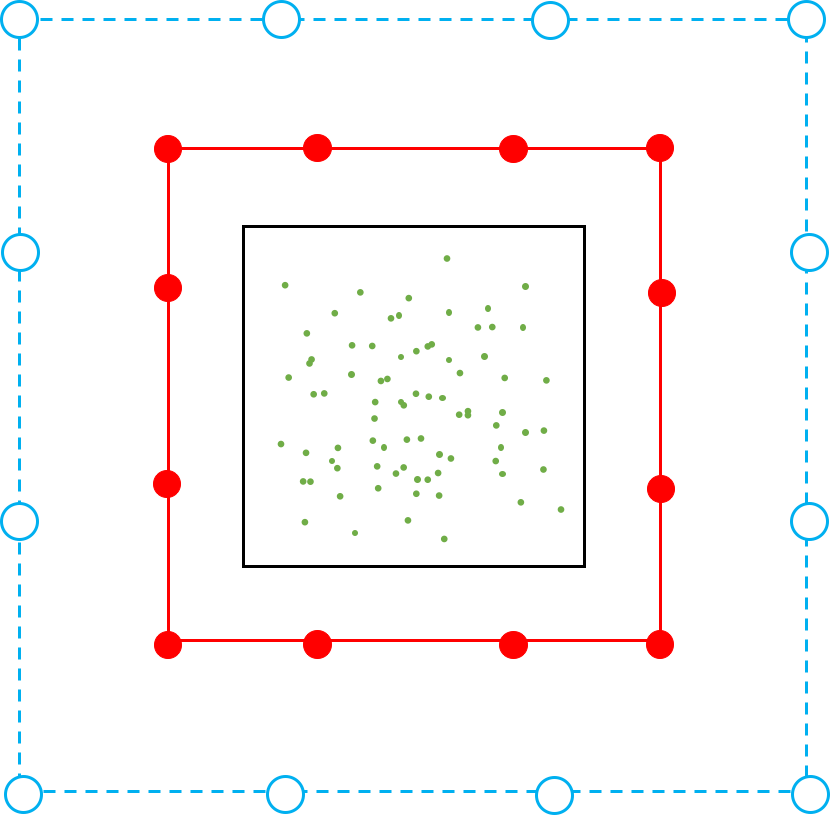
\includegraphics[width=0.3\textwidth]{introduction/upward_surface.png}}
    \hfill
  {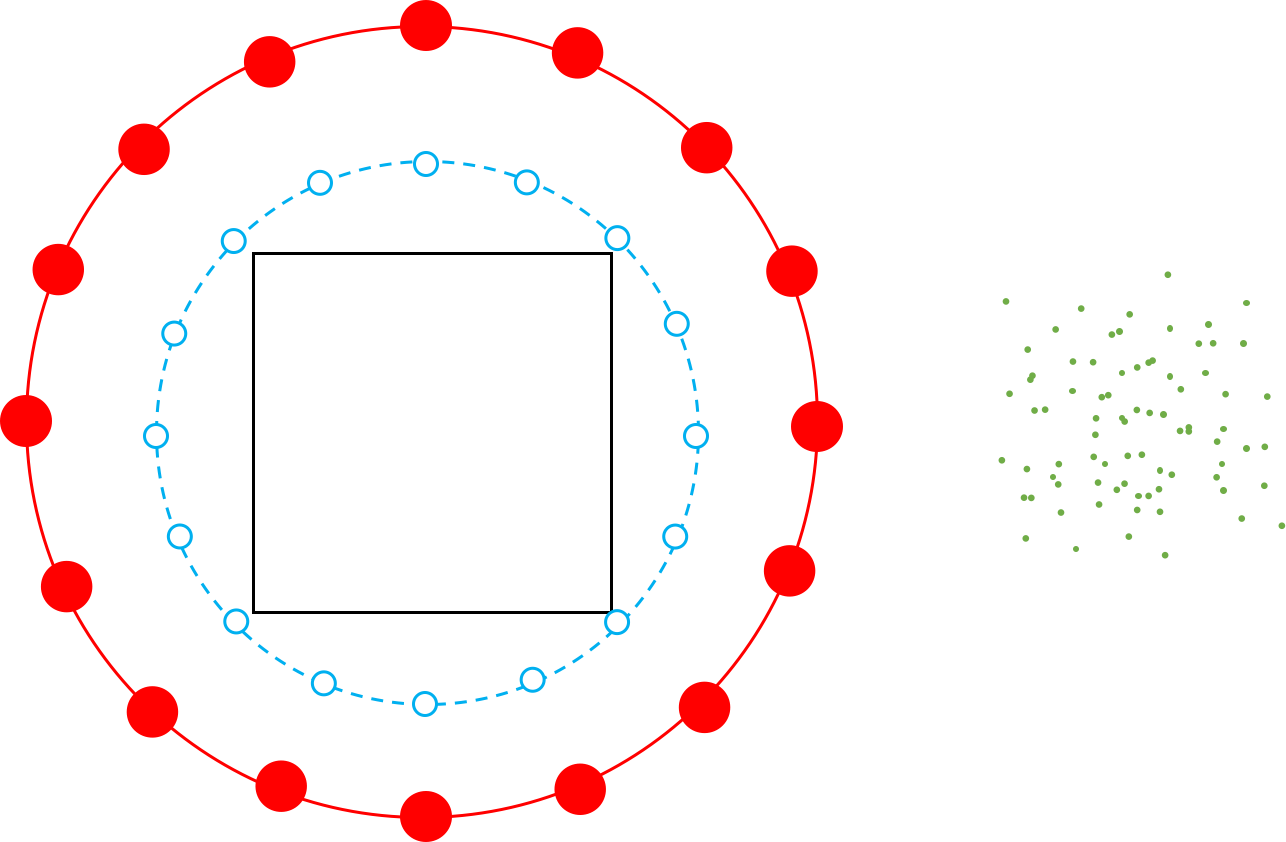
\includegraphics[width=0.4\textwidth]{introduction/downward_surface.png}}
  \vspace{0pt}
  \caption{Cross section of three dimensional cubic upward/downward equivalent and
    check surfaces. Source points are denoted by green circles. Red solid lines
    denote equivalent surfaces, and blue checked lines denote check surfaces. This
    figure is adapted directly from \cite{Ying:2004:JCP}.}

  \label{fig:1_2_upward_downward_surfaces}
\end{figure}


\begin{figure}[!h]
    \centering
    {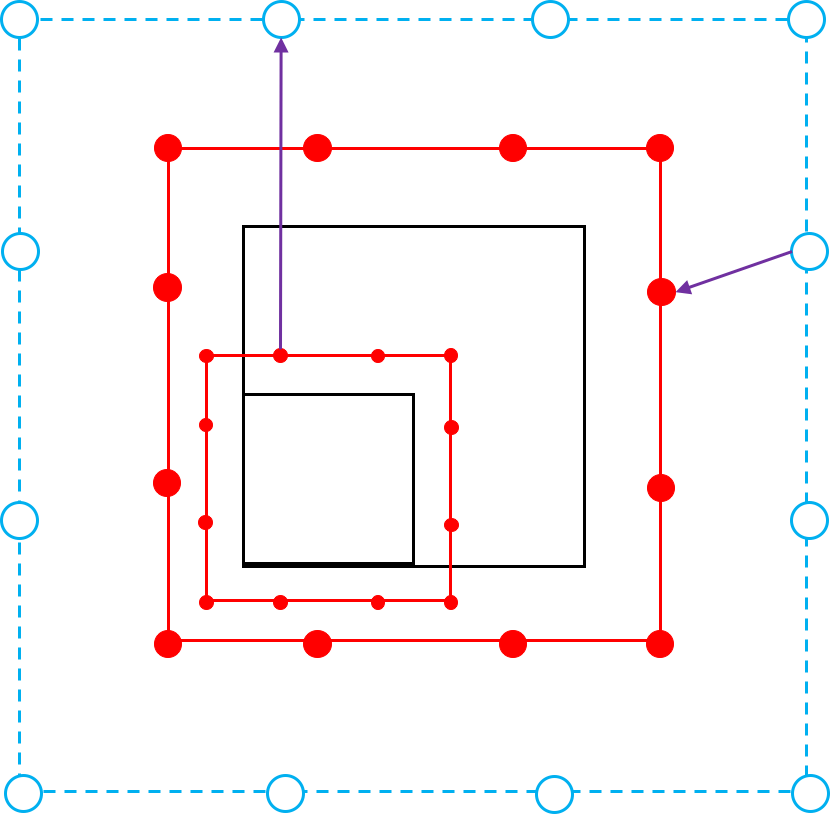
\includegraphics[width=0.4\textwidth]{introduction/kifmm_m2m.png}}
    \hfill
  {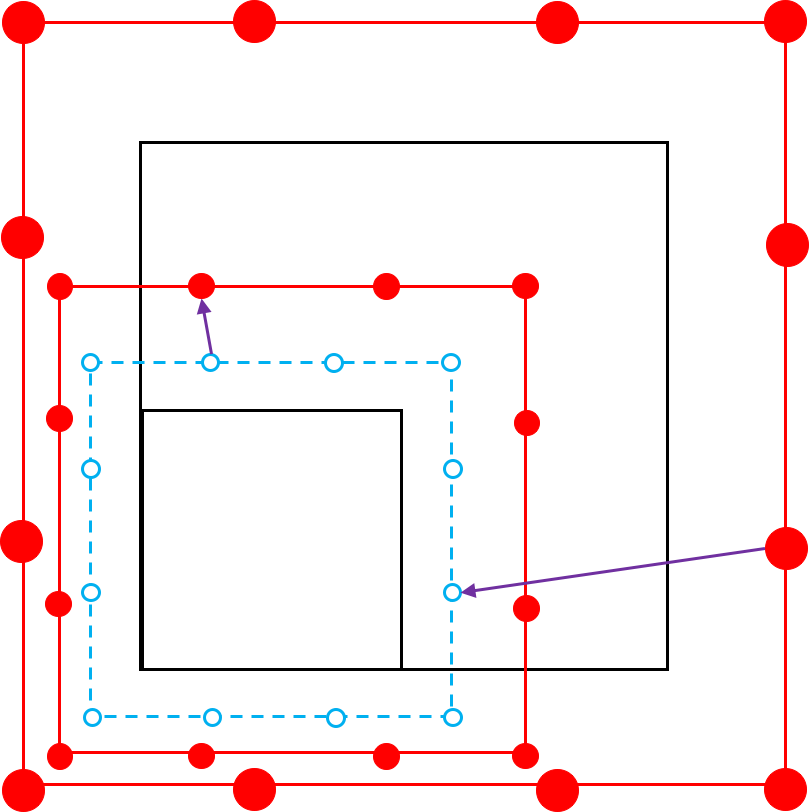
\includegraphics[width=0.4\textwidth]{introduction/kifmm_l2l.png}}
  \vspace{0pt}
  \caption{Foo bar}

  \label{fig:1_2_m2m_l2l}
\end{figure}


\begin{figure}[!h]
    \centering
    {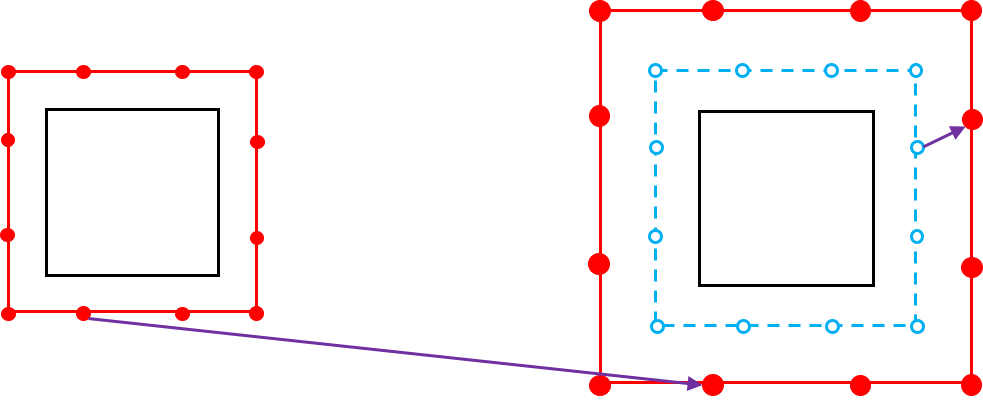
\includegraphics[width=\textwidth]{introduction/kifmm_m2l.png}}
    \caption{Foo bar}
  \label{fig:1_2_m2l}
\end{figure}


\subsection{Algorithm Structure \& Analysis}


\subsection{Summary}

